
\documentclass[letterpaper,hide notes,xcolor={table,svgnames},pdftex,10pt]{beamer}
\def\showexamples{t}


%\usepackage[svgnames]{xcolor}

%% Demo talk
%\documentclass[letterpaper,notes=show]{beamer}

\usecolortheme{crane}
\setbeamertemplate{navigation symbols}{}

\usetheme{MyPittsburgh}
%\usetheme{Frankfurt}

%\usepackage{tipa}

\usepackage{hyperref}
\usepackage{graphicx,xspace}
\usepackage[normalem]{ulem}
\usepackage{multicol}
\usepackage{amsmath,amssymb,amsthm,graphicx,xspace}
\newcommand\SF[1]{$\bigstar$\footnote{SF: #1}}

\usepackage[default]{sourcesanspro}
\usepackage[T1]{fontenc}
\usepackage[scaled]{beramono}
\usepackage{tikzpagenodes}

\newcounter{tmpnumSlide}
\newcounter{tmpnumNote}


% old question code
%\newcommand\question[1]{{$\bigstar$ \small \onlySlide{2}{#1}}}
% \newcommand\nquestion[1]{\ifdefined \presentationonly \textcircled{?} \fi \note{\par{\Large \textbf{?}} #1}}
% \newcommand\nanswer[1]{\note{\par{\Large \textbf{A}} #1}}


 \newcommand\mnote[1]{%
   \addtocounter{tmpnumSlide}{1}
   \ifdefined\showcues {~\tiny\fbox{\arabic{tmpnumSlide}}}\fi
   \note{\setlength{\parskip}{1ex}\addtocounter{tmpnumNote}{1}\textbf{\Large \arabic{tmpnumNote}:} {#1\par}}}

\newcommand\mmnote[1]{\note{\setlength{\parskip}{1ex}#1\par}}

%\newcommand\mnote[2][]{\ifdefined\handoutwithnotes {~\tiny\fbox{#1}}\fi
% \note{\setlength{\parskip}{1ex}\textbf{\Large #1:} #2\par}}

%\newcommand\mnote[2][]{{\tiny\fbox{#1}} \note{\setlength{\parskip}{1ex}\textbf{\Large #1:} #2\par}}

\newcommand\mquestion[2]{{~\color{red}\fbox{?}}\note{\setlength{\parskip}{1ex}\par{\Large \textbf{?}} #1} \note{\setlength{\parskip}{1ex}\par{\Large \textbf{A}} #2\par}\ifdefined \presentationonly \pause \fi}

\newcommand\blackboard[1]{%
\ifdefined   \showblackboard
  {#1}
  \else {\begin{center} \fbox{\colorbox{blue!30}{%
         \begin{minipage}{.95\linewidth}%
           \hspace{\stretch{1}} Some space intentionally left blank; done at the blackboard.%
         \end{minipage}}}\end{center}}%
         \fi%
}



%\newcommand\q{\tikz \node[thick,color=black,shape=circle]{?};}
%\newcommand\q{\ifdefined \presentationonly \textcircled{?} \fi}

\usepackage{listings}
\lstset{basicstyle=\footnotesize\ttfamily,
	breaklines=true,
	aboveskip=15pt,
  	belowskip=15pt,
	frame=lines,
	numbers=left, basicstyle=\scriptsize, numberstyle=\tiny, stepnumber=0, numbersep=2pt
}

\usepackage{siunitx}
\newcommand\sius[1]{\num[group-separator = {,}]{#1}\si{\micro\second}}
\newcommand\sims[1]{\num[group-separator = {,}]{#1}\si{\milli\second}}
\newcommand\sins[1]{\num[group-separator = {,}]{#1}\si{\nano\second}}
\sisetup{group-separator = {,}, group-digits = true}

%% -------------------- tikz --------------------
\usepackage{tikz}
\usetikzlibrary{positioning}
\usetikzlibrary{arrows,backgrounds,automata,decorations.shapes,decorations.pathmorphing,decorations.markings,decorations.text,decorations.pathreplacing}

\tikzstyle{place}=[circle,draw=blue!50,fill=blue!20,thick, inner sep=0pt,minimum size=6mm]
\tikzstyle{transition}=[rectangle,draw=black!50,fill=black!20,thick, inner sep=0pt,minimum size=4mm]

\tikzstyle{block}=[rectangle,draw=black, thick, inner sep=5pt]
\tikzstyle{bullet}=[circle,draw=black, fill=black, thin, inner sep=2pt]

\tikzstyle{pre}=[<-,shorten <=1pt,>=stealth',semithick]
\tikzstyle{post}=[->,shorten >=1pt,>=stealth',semithick]
\tikzstyle{bi}=[<->,shorten >=1pt,shorten <=1pt, >=stealth',semithick]

\tikzstyle{mut}=[-,>=stealth',semithick]

\tikzstyle{treereset}=[dashed,->, shorten >=1pt,>=stealth',thin]

\usepackage{ifmtarg}
\usepackage{xifthen}
\makeatletter
% new counter to now which frame it is within the sequence
\newcounter{multiframecounter}
% initialize buffer for previously used frame title
\gdef\lastframetitle{\textit{undefined}}
% new environment for a multi-frame
\newenvironment{multiframe}[1][]{%
\ifthenelse{\isempty{#1}}{%
% if no frame title was set via optional parameter,
% only increase sequence counter by 1
\addtocounter{multiframecounter}{1}%
}{%
% new frame title has been provided, thus
% reset sequence counter to 1 and buffer frame title for later use
\setcounter{multiframecounter}{1}%
\gdef\lastframetitle{#1}%
}%
% start conventional frame environment and
% automatically set frame title followed by sequence counter
\begin{frame}%
\frametitle{\lastframetitle~{\normalfont(\arabic{multiframecounter})}}%
}{%
\end{frame}%
}
\makeatother

\makeatletter
\newdimen\tu@tmpa%
\newdimen\ydiffl%
\newdimen\xdiffl%
\newcommand\ydiff[2]{%
    \coordinate (tmpnamea) at (#1);%
    \coordinate (tmpnameb) at (#2);%
    \pgfextracty{\tu@tmpa}{\pgfpointanchor{tmpnamea}{center}}%
    \pgfextracty{\ydiffl}{\pgfpointanchor{tmpnameb}{center}}%
    \advance\ydiffl by -\tu@tmpa%
}
\newcommand\xdiff[2]{%
    \coordinate (tmpnamea) at (#1);%
    \coordinate (tmpnameb) at (#2);%
    \pgfextractx{\tu@tmpa}{\pgfpointanchor{tmpnamea}{center}}%
    \pgfextractx{\xdiffl}{\pgfpointanchor{tmpnameb}{center}}%
    \advance\xdiffl by -\tu@tmpa%
}
\makeatother
\newcommand{\copyrightbox}[3][r]{%
\begin{tikzpicture}%
\node[inner sep=0pt,minimum size=2em](ciimage){#2};
\usefont{OT1}{phv}{n}{n}\fontsize{4}{4}\selectfont
\ydiff{ciimage.south}{ciimage.north}
\xdiff{ciimage.west}{ciimage.east}
\ifthenelse{\equal{#1}{r}}{%
\node[inner sep=0pt,right=1ex of ciimage.south east,anchor=north west,rotate=90]%
{\raggedleft\color{black!50}\parbox{\the\ydiffl}{\raggedright{}#3}};%
}{%
\ifthenelse{\equal{#1}{l}}{%
\node[inner sep=0pt,right=1ex of ciimage.south west,anchor=south west,rotate=90]%
{\raggedleft\color{black!50}\parbox{\the\ydiffl}{\raggedright{}#3}};%
}{%
\node[inner sep=0pt,below=1ex of ciimage.south west,anchor=north west]%
{\raggedleft\color{black!50}\parbox{\the\xdiffl}{\raggedright{}#3}};%
}
}
\end{tikzpicture}
}


%% --------------------

%\usepackage[excludeor]{everyhook}
%\PushPreHook{par}{\setbox0=\lastbox\llap{MUH}}\box0}

%\vspace*{\stretch{1}

%\setbox0=\lastbox \llap{\textbullet\enskip}\box0}

\setlength{\parskip}{\fill}

\newcommand\noskips{\setlength{\parskip}{1ex}}
\newcommand\doskips{\setlength{\parskip}{\fill}}

\newcommand\xx{\par\vspace*{\stretch{1}}\par}
\newcommand\xxs{\par\vspace*{2ex}\par}
\newcommand\tuple[1]{\langle #1 \rangle}
\newcommand\code[1]{{\sf \footnotesize #1}}
\newcommand\ex[1]{\uline{Example:} \ifdefined \presentationonly \pause \fi
  \ifdefined\showexamples#1\xspace\else{\uline{\hspace*{2cm}}}\fi}

\newcommand\ceil[1]{\lceil #1 \rceil}


\AtBeginSection[]
{
   \begin{frame}
       \frametitle{Outline}
       \tableofcontents[currentsection]
   \end{frame}
}



\pgfdeclarelayer{edgelayer}
\pgfdeclarelayer{nodelayer}
\pgfsetlayers{edgelayer,nodelayer,main}

\tikzstyle{none}=[inner sep=0pt]
\tikzstyle{rn}=[circle,fill=Red,draw=Black,line width=0.8 pt]
\tikzstyle{gn}=[circle,fill=Lime,draw=Black,line width=0.8 pt]
\tikzstyle{yn}=[circle,fill=Yellow,draw=Black,line width=0.8 pt]
\tikzstyle{empty}=[circle,fill=White,draw=Black]
\tikzstyle{bw} = [rectangle, draw, fill=blue!20, 
    text width=4em, text centered, rounded corners, minimum height=2em]
    
    \newcommand{\CcNote}[1]{% longname
	This work is licensed under the \textit{Creative Commons #1 3.0 License}.%
}
\newcommand{\CcImageBy}[1]{%
	\includegraphics[scale=#1]{creative_commons/cc_by_30.pdf}%
}
\newcommand{\CcImageSa}[1]{%
	\includegraphics[scale=#1]{creative_commons/cc_sa_30.pdf}%
}
\newcommand{\CcImageNc}[1]{%
	\includegraphics[scale=#1]{creative_commons/cc_nc_30.pdf}%
}
\newcommand{\CcGroupBySa}[2]{% zoom, gap
	\CcImageBy{#1}\hspace*{#2}\CcImageNc{#1}\hspace*{#2}\CcImageSa{#1}%
}
\newcommand{\CcLongnameByNcSa}{Attribution-NonCommercial-ShareAlike}

\newenvironment{changemargin}[1]{% 
  \begin{list}{}{% 
    \setlength{\topsep}{0pt}% 
    \setlength{\leftmargin}{#1}% 
    \setlength{\rightmargin}{1em}
    \setlength{\listparindent}{\parindent}% 
    \setlength{\itemindent}{\parindent}% 
    \setlength{\parsep}{\parskip}% 
  }% 
  \item[]}{\end{list}} 




\title{Lecture 30 ---Profiling and Scalability}

\author{Jeff Zarnett\\ \small \texttt{jzarnett@uwaterloo.ca}}
\institute{Department of Electrical and Computer Engineering \\
  University of Waterloo}
\date{\today}


\begin{document}

\begin{frame}
  \titlepage

 \end{frame}



\begin{frame}
\frametitle{Profiling and Scalability}

\Large
\begin{changemargin}{2cm}
Goal: scale number of users,

\[ 1 \rightarrow 100 \rightarrow 10 000 000. \]

Be more fast? \\
You have other options too\ldots
\end{changemargin}

\end{frame}


\begin{frame}
\frametitle{Don't Guess, Measure}

\large
\begin{changemargin}{2cm}
As always, we want to measure (profile).\\[1em]
3 principles to think about\\
when going from dev to production:
\end{changemargin}

\end{frame}



\begin{frame}
\frametitle{Hardware Principle}

\large
\begin{changemargin}{2cm}
Scalability testing $\neq$  QA testing.\\[1em]

Dev + QA on local computer.\\
Your concerns: Is it right? Is it fast enough?\\[1em]

Fine, but it's no way to test if it scales. 
\end{changemargin}

\end{frame}



\begin{frame}
\frametitle{Hardware Principle}

\large
\begin{changemargin}{2cm}
Test on prod-like machines.\\[1em]
Low-end systems have very different limiting factors. \\[1em]
Your laptop: limited by 8GB of RAM.\\
Prod server: 64GB of RAM.\\[1em]
So you might spend a great deal of time worrying about RAM usage and it just doesn't matter.
\end{changemargin}

\end{frame}



\begin{frame}
\frametitle{Reality Principle}
\large
\begin{changemargin}{2cm}
Use a ``real'' workload.\\
(As far as possible).\\[1em]
Maybe not actual live customer data,\\
but try to come close.\\[1em]
Limited test data/scenarios $\Rightarrow$ \\
\qquad inaccurate test results.\\[1em]
Your tests run summary reports occasionally\ldots\\
your users might run them every hour. 
\end{changemargin}
\end{frame}



\begin{frame}
\frametitle{Volume Principle}
\large
\begin{changemargin}{2cm}
``More is the new more.'' 

Lighter workloads OK for regression testing. 

To see how your system performs under pressure, you actually need to put it under pressure. 

Can simulate pressure by limiting RAM or\\ running something very CPU-intensive concurrently,\\
but it's just not the same.

These tests also  of great interest to the customers, who would like to know that you can deliver. 
\end{changemargin}

\end{frame}



\begin{frame}
\frametitle{Reproducibility and Regression Testing}

\large
\begin{changemargin}{2cm}
Science rule 1: results need to be reproducible!

Good programming practice: must run unit tests,\\
and re-run to make sure it all works. 

Old (solved) performance issues also bad.

Or a new change that slows the whole program down still more bad.
\end{changemargin}
\end{frame}



\begin{frame}
\frametitle{Characterizing Problems}

\large
\begin{changemargin}{2cm}
Example: application deployed on two systems---application server and database server. 

Data stored on an external SAN \\
with RAID0 configuration. 

Java program simulated object creation\\
with 15 threads. 

Performance metric: objects created per second. 
\end{changemargin}

\end{frame}



\begin{frame}
\frametitle{Scalability Fail(ability)}

\begin{center}
	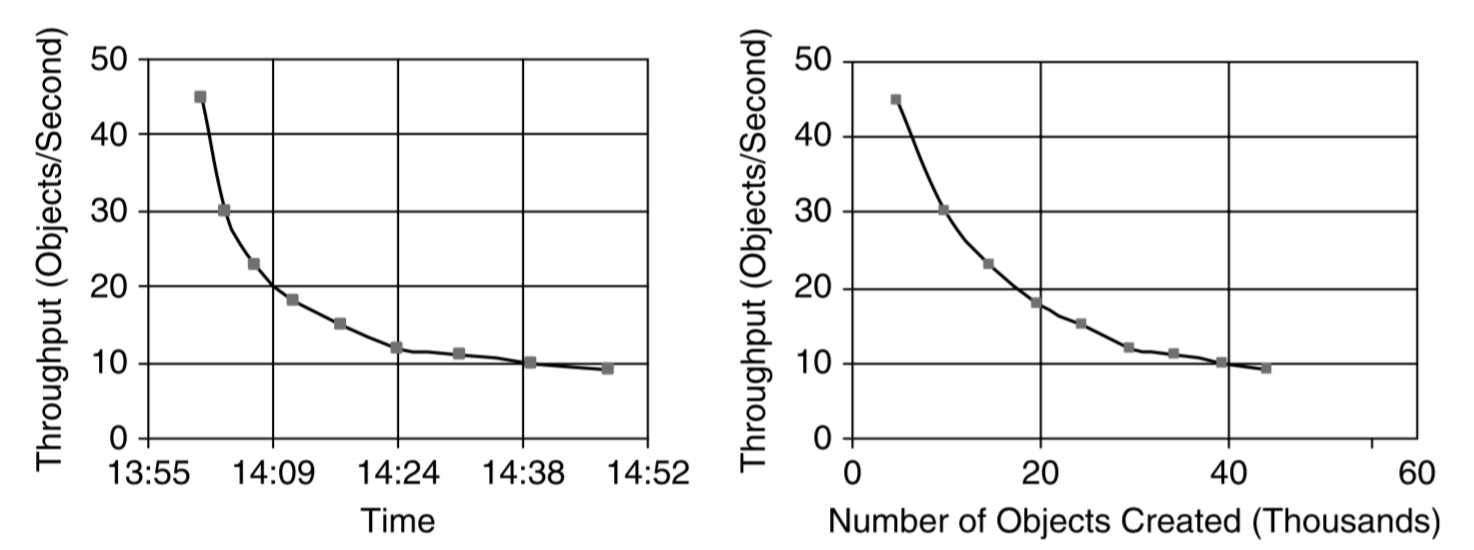
\includegraphics[width=0.85\textwidth]{images/batch-job-scalability.png}
\end{center}

\Large
\begin{changemargin}{1cm}
This is, to use the technical term, ``not good''.
\end{changemargin}
\end{frame}



\begin{frame}
\frametitle{Elementary, My Dear Watson!}

\Large
\begin{changemargin}{1cm}
\begin{quote}
\textit{It is a capital mistake to theorize before one has data. Insensibly one begins to twist facts to suit theories, instead of theories to suit facts.}
\end{quote}
\hfill --- Sherlock Holmes\\
\hfill (\textit{A Scandal in Bohemia}; Sir Arthur Conan Doyle)
\end{changemargin}
\end{frame}



\begin{frame}
\frametitle{Collect Evidence}

\Large
\begin{changemargin}{1cm}
Who's to blame?
\begin{enumerate}
	\item CPU
	\item Memory
	\item Disk
	\item Network
\end{enumerate}

These are, obviously, \\
categories rather than specific causes.
\end{changemargin}
\end{frame}



\begin{frame}
\frametitle{Blame the CPU}

\large
\begin{changemargin}{1cm}
CPU is probably the easiest of these to diagnose. \\[1em]
\texttt{htop}, Task Manager, etc. will tell you if CPU hosed.\\
Look at the \%CPU columns\\
and see where all your CPU is going. 
\end{changemargin}


\end{frame}



\begin{frame}[fragile]
\frametitle{Felicity Smoak, ``Overwatch'' (Oracle was taken)}

\large
\begin{changemargin}{1cm}
Still, that tells you about right now; \\
what about the long term average? \\[1em]

Checking with my machine ``Loki'', that donates its free CPU cycles to world community grid (I'm singlehandedly saving the world, you see.):\\[1em]

{\scriptsize
\begin{verbatim}
top - 07:28:19 up 151 days, 23:38,  8 users,  load average: 0.87, 0.92, 0.91
\end{verbatim}
}

Those last three numbers are the one, five, and fifteen minute averages of CPU load, respectively. \\[1em]

Lower numbers mean less CPU usage and a less busy machine. 
\end{changemargin}

\end{frame}




\begin{frame}
\frametitle{Interpreting Load Numbers}

\large
\begin{changemargin}{1cm}
Picture a single core of a CPU as a lane of traffic. 

You are a bridge operator and so you need to monitor how many cars are waiting to cross that bridge. 

If no cars are waiting, traffic is good and drivers are happy. 

If there is a backup of cars, then there will be delays.
\end{changemargin}

\end{frame}



\begin{frame}
\frametitle{Single-CPU Load Scheme}

\large
\begin{changemargin}{1cm}
\begin{enumerate}
	\item 0.00 means no traffic. \\
    Anything between 0.00 and 0.99 means we're under capacity and there will be no delay.\\[1em]
	\item 1.00 means we are exactly at capacity. \\
    Everything is okay, but if one more car shows up, there will be a delay.\\[1em]
	\item Anything above 1.00 means there's a backup (delay). \\
    If we have 2.00 load, then the bridge is full and there's an equal number of cars waiting to get on the bridge. 
\end{enumerate}
\end{changemargin}

\end{frame}



\begin{frame}
\frametitle{Car Analogy}

\begin{center}
	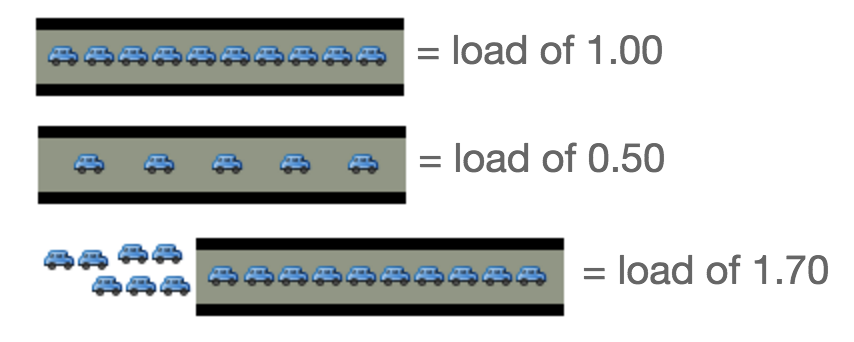
\includegraphics[width=\textwidth]{images/car-analogy.png}
\end{center}

\end{frame}



\begin{frame}
\frametitle{Is it a Problem?}

\large
\begin{changemargin}{1cm}
$\ge$ 1.00 isn't necessarily bad, but you should be concerned if there is consistent load of 1.00 or above. 

$<$ 1.00 but getting close to it: you know how much room you have to scale things up.

$>$ 0.70 then it's probably time to investigate.

$\ge$ 1.00 consistently we have a serious problem. 

5.00: this is a red alert situation.
\end{changemargin}

\end{frame}



\begin{frame}
\frametitle{Multicore}

\large
\begin{changemargin}{1cm}
Now this is for a single CPU---if you have a load of 3.00 and a quad core CPU, this is okay. 

Traffic analogy: four lanes of traffic, of which 3 are being used to capacity.

So we have a fourth lane free and it's as if we're at 75\% utilization on a single CPU.
\end{changemargin}

\end{frame}



\begin{frame}
\frametitle{End Digression}


\large
\begin{changemargin}{1cm}
Back to our example. Is it CPU? 

The Application Server CPU utilization, on average, \\
was about 10\% and on the database server, about 36\%. 

So that is probably not the cause. 

Next on the list is memory. 
\end{changemargin}
\end{frame}



\begin{frame}[fragile]
\frametitle{Disk? Or Memory?}

\large
\begin{changemargin}{1cm}
How to tell? Look at disk utilization. \\[1em]

Not enough RAM $\Rightarrow$ swapping, bad perf, no scalability.\\[1em]

(In the worst case.)\\[1em]

You can ask via \texttt{top} about how much swap is being used, but that's probably not the interesting value. 

{\scriptsize
\begin{verbatim}
KiB Mem:   8167736 total,  6754408 used,  1413328 free,   172256 buffers
KiB Swap:  8378364 total,  1313972 used,  7064392 free.  2084336 cached Mem
\end{verbatim}
}
\end{changemargin}

\end{frame}



\begin{frame}
\frametitle{Misleading Memory}

\large
\begin{changemargin}{1cm}
Why? Memory being ``full'' does not necessarily mean anything bad. \\[1em]

It means the resource is being used to its maximum potential, yes, but there is no benefit to keeping a block of memory open for no reason. (Or stockpiling late days).\\[1em]

Also, memory is unlike CPU; if there's nothing for the CPU to do, it will just idle (low power state).
\end{changemargin}

\end{frame}


\begin{frame}
\frametitle{Really, Dvorak, Really?}

\large
\begin{changemargin}{1cm}
Memory won't ``forget'' data if it doesn't happen to be needed right now---data will hang around in memory until there is a reason to move or change it. 

So freaking out about memory appearing as full is kind of like getting all in a knot about how ``System Idle Process'' is hammering the CPU\ldots
\end{changemargin}

\end{frame}




\begin{frame}
\frametitle{Page Faults}

\large
\begin{changemargin}{1cm}
You can also ask about page faults, with the command
\begin{center}
\texttt{ps -eo min\_flt,maj\_flt,cmd}
\end{center}

Major page faults: had to fetch from disk. 

Minor page faults: had to copy a page from another process. 

The output of this is too big even for the notes.

This is process-lifetime data.
\end{changemargin}
\end{frame}



\begin{frame}[fragile]
\frametitle{Swapping Report}

\Large
\begin{changemargin}{1cm}
What you really want is to ask Linux for a report on swapping:
\end{changemargin}
\vspace*{-2em}
{\scriptsize
\begin{verbatim}
jz@Loki:~$ vmstat 5
procs -----------memory---------- ---swap-- -----io---- -system-- ------cpu-----
 r  b   swpd   free   buff  cache   si   so    bi    bo   in   cs us sy id wa st
 1  0 1313972 1414600 172232 2084296    0    0     3    39    1    1 27  1 72  0  0
 0  0 1313972 1414476 172232 2084296    0    0     0    21  359  735 19  0 80  0  0
 0  0 1313972 1414656 172236 2084228    0    0     0   102  388  758 22  0 78  0  0
 4  0 1313972 1414592 172240 2084292    0    0     0    16  501  847 33  0 67  0  0
 0  0 1313972 1412028 172240 2084296    0    0     0     0  459  814 29  0 71  0  0
\end{verbatim}
}

\end{frame}



\begin{frame}[fragile]
\frametitle{Swapping Report with Actual Swapping}

{\small
\begin{verbatim}
  procs                      memory    swap          io     system cpu
r  b  w   swpd   free  buff cache  si  so   bi   bo   in    cs us  sy  id
. . .
1  0  0  13344   1444  1308 19692   0 168  129   42 1505   713 20  11  69
1  0  0  13856   1640  1308 18524  64 516  379  129 4341   646 24  34  42
3  0  0  13856   1084  1308 18316  56  64   14    0  320  1022 84   9   8
\end{verbatim}
}

\end{frame}



\begin{frame}
\frametitle{Skip to Disk}

\large
\begin{changemargin}{1cm}
Looking at disk might seem slightly redundant if memory is not the limiting factor. 

After all, if the data were in memory it would be unnecessary to go to disk in the first place. 

Still, sometimes we can take a look at the disk and see if that is our bottleneck.
\end{changemargin}

\end{frame}




\begin{frame}[fragile]
\frametitle{Looking at Disk Usage}

{\tiny
\begin{verbatim}
jz@Loki:~$ iostat -dx /dev/sda 5 
Linux 3.13.0-24-generic (Loki) 	16-02-13 	_x86_64_	(4 CPU)

Device:         rrqm/s   wrqm/s     r/s     w/s    rkB/s    wkB/s avgrq-sz avgqu-sz   await r_await w_await  svctm  %util
sda               0.24     2.78    0.45    2.40    11.60   154.98   116.91     0.17   61.07   11.57   70.27   4.70   1.34
\end{verbatim}
}

\large
\begin{changemargin}{1cm}
Last column \%util tells us what we want to know.
\end{changemargin}

\end{frame}



\begin{frame}[fragile]
\frametitle{Network}

\large
\begin{changemargin}{1cm}
We can ask about the network with \texttt{nload}. 
 
You get a nice little graph if there is anything to see. 

But you'll get the summary, at least:

\begin{verbatim}
Curr: 3.32 kBit/s
Avg: 2.95 kBit/s
Min: 1.02 kBit/s
Max: 12.60 kBit/s
Ttl: 39.76 GByte                                                                                       \end{verbatim}
\end{changemargin}
\end{frame}



\begin{frame}
\frametitle{Back to the Original Question}

\large
\begin{changemargin}{1cm}
The book contains the full story, which is maybe interesting to you if you wanted to dig into the specifics about Oracle 10g and SQL query syntax. 

You probably don't care about the details, \\
but 96.4\% of the total database call time was attributed to database CPU
\end{changemargin}

\end{frame}



\begin{frame}[fragile]
\frametitle{Top 5 Queries}

\large
\begin{changemargin}{1cm}
Sure enough, the ``top 5'' queries were taking up a huge amount of time and they all look something like:
\end{changemargin}
\begin{verbatim}
SELECT documentId, classId, dataGroupId, consistencyId 
FROM objectTable 
WHERE objectID = <value>;
\end{verbatim}

\large
\begin{changemargin}{1cm}
Why does performance of this stink?
\end{changemargin}

\end{frame}



\begin{frame}
\frametitle{Top 5 Query Performance}

\large
\begin{changemargin}{1cm}
Lots of reads from the database. 

The reads themselves don't necessarily go to disk (cache/buffers/etc may save us here) but we're still doing a lot of reads of data. 

To speed this up, what we need is to add an additional index for each of these tables. 

This is one of the strategies we've talked about before---``be prepared''.
\end{changemargin}


\end{frame}



\begin{frame}
\frametitle{The Impact of the Index}

\begin{center}
	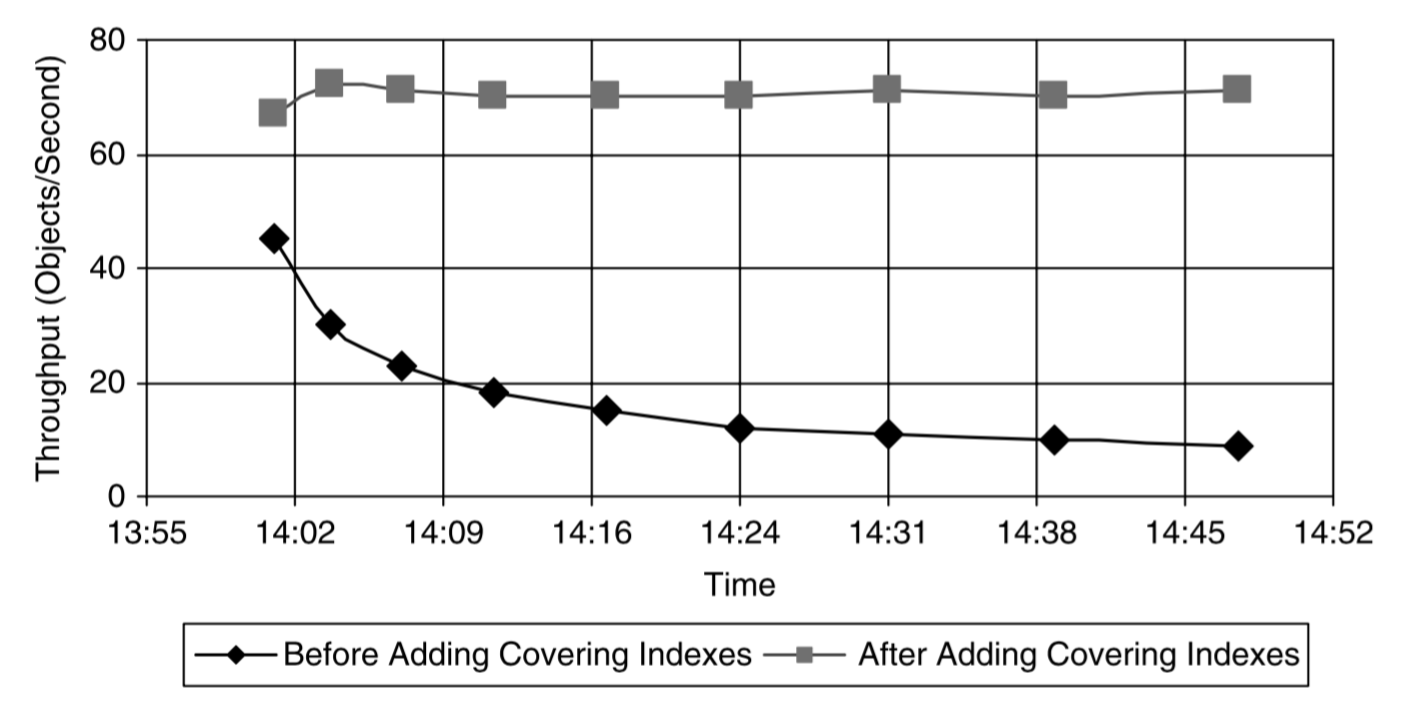
\includegraphics[width=0.85\textwidth]{images/adding-indexes.png}
\end{center}

\end{frame}

\end{document}

